\section{Bohreinrichtung}
\subsection{Lastenheft}
Die in Abbildung \ref{fig:Bohreinrichtung} dargestellte Bohreinrichtung verfügt über zwei Schalter S1 und S2. Diese stellen die Bedienung dar. Wird der Schalter eins  betätigt, soll der automatische Ablauf aus der Grundstellung heraus beginnen. Zuerst bewegt sich Zylinder eins in Arbeitsstellung und spannt das Werkstück ein. Anschließend startet der Bohrer und Zylinder zwei fährt aus und ermöglicht den eigentlichen Bohrvorgang. Am tiefsten Punkt soll der Bohrkopf für zwei Sekunden im Werkstück verbleiben und anschließend wieder einfahren. Zum Schluss fährt Zylinder eins wieder in die Grundstellung und gibt damit das Werkstück frei. Schalter S2 dient dazu, die Anlage aus jeder beliebigen Position in die Grundstellung zu bewegen.
\begin{figure}[H]
   \centering
    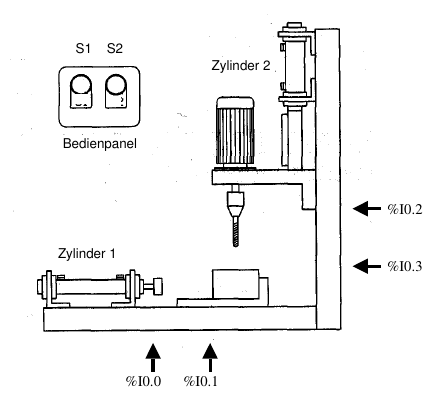
\includegraphics[scale=0.65]{Bilder/Aufgabenstellung.png}
    \caption[Bohreinrichtung]{Modell der Bohreinrichtung
    \footnotemark}
    \label{fig:Bohreinrichtung}
\end{figure}
\footnotetext{\cite{Riege}}
In Tabelle \ref{tab:Adressen}, Seite \pageref{tab:Adressen} sind die Adressen der Ein- und Ausgänge festgelegt. Hierbei steht \%Qx.X für Aktuatoren (Ausgang) und \%Ix.X für Sensoren (Eingang). 
In der Aufgabenstellung wurde der Bohrantrieb nicht als Aktuator erwähnt, eine Adresszuweisung erfolgt ebenso nicht. Deshalb wird die Adresse auf \%Q1.4 festgelegt. Zudem würde der Bohrer laut Aufgabenstellung ohne Drehbewegung in das Werkstück fahren. Das hätte zur Folge, dass Bohrer und Werkstück beschädigt bzw. zerstört werden. Aus diesem Grund wurde im oberen Abschnitt festgelegt, dass vor dem Betätigen des Zylinders zwei der Bohrantrieb bereits aktiv sein soll.
\begin{table}[h]
    %\rowcolors{2}{lightgray}{}
    \centering
\begin{tabular}{|p{2.5cm}|p{2.5cm}|p{1.5cm}|}
    \rowcolor{gray}
    \hline
    \multicolumn{2}{|c|}{\textbf{Benennung}} &  \textbf{Adresse}\\
    \hline
    \multirow{2}{4em}{Schalter} & S1 & \%I0.4 \\
    & S2 & \%I0.5 \\
    \hline
    \multirow{4}{5em}{Zylinder 1} & Anfangspos. & \%I0.0 \\
    & Endpos. & \%I0.1 \\
    & ausfahren & \%Q1.0 \\
    & einfahren & \%Q1.1 \\
    \hline
    \multirow{4}{5em}{Zylinder 2} & Anfangspos. & \%I0.2 \\
    & Endpos. & \%I0.3 \\
    & ausfahren & \%Q1.2 \\
    & einfahren & \%Q1.3 \\
    \hline
    \multicolumn{2}{|l|}{Bohrantrieb} & \%Q1.4 \\
    \hline
\end{tabular}
    \caption{Adressen der Sensoren und Aktoren}
    \label{tab:Adressen}
\end{table}\\
Die beschriebene Schrittabfolge soll mithilfe der Entwicklungsumgebung \ac{codesys} in \ac{fup} erstellt werden. Anschließend soll das erstellte Programm in einer Simulation auf Funktion überprüft werden.
Auf weitere technische und wirtschaftliche Aspekte, die für ein Lastenheft notwendig sind, wird nicht weiter eingegangen, da es für das Assignment nicht gefordert wird.
%-----------------------------------------------------------------------------------------------
%-----------------------------------------------------------------------------------------------
\subsection{Programmablaufplan}
Steuerungs- und Regelabläufe lassen sich in unterschiedlichen Modellen darstellen. Schalt- oder Ablaufpläne, Diagramme und Graphen sind Beispiele zur unterschiedlichen Visualisierung von technischen Abläufen. Je nach Umfang des zu realisierenden Systems sind in der Regel mehrere verschiedene Modelle notwendig.\autocite[vgl.][1446]{Boege2021}\\
Der im Lastenheft beschriebene Bohrvorgang wird in einem Programmablaufplan grafisch beschrieben. Ein Ausschnitt ist in Abbildung \ref{fig:Ausschnitt_pap}, Seite \pageref{fig:Ausschnitt_pap} dargestellt. Für die Erläuterung der Verschaltung der Aktoren, Sensoren und \ac{sps}-Einheit ist ein Stromlaufplan notwendig. Das ist in diesem Assignment jedoch nicht gefordert.\\
\begin{figure}[H]
   \centering
    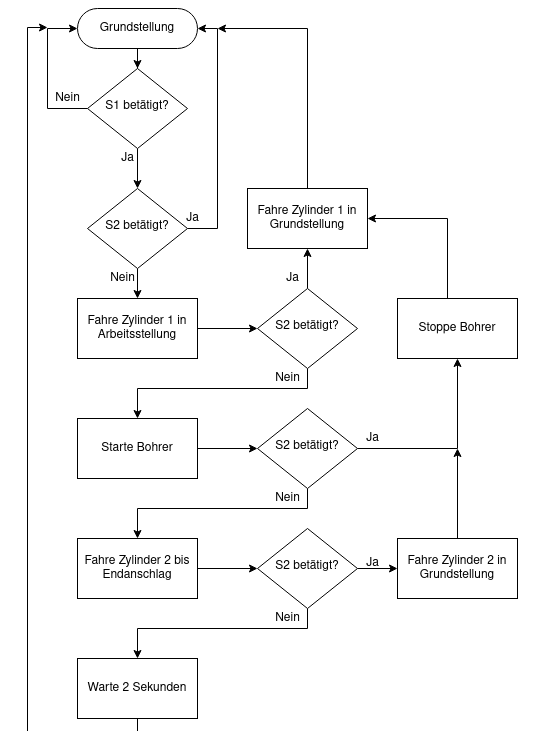
\includegraphics[scale=0.75]{Bilder/Flow_Chart_Bohrvorrichtung_Ausschnitt.png}
    \caption[Ausschnitt Programmablaufplan]{Ausschnitt vom Programmablaufplan (eigener Entwurf)}
    \label{fig:Ausschnitt_pap}
\end{figure}
Die Startbedingung für das System ist die Grundstellung aller Aktoren. Durch das Drücken von S2 kann die Grundstellung angefahren werden. Nach dem Auslösen von S1 kann der Ablauf aus der Grundstellung heraus gestartet werden. Während jeder Anweisung wird überprüft, ob S2 betätigt wird. Ist das der Fall, wird die Schrittkette rückwärts durchlaufen, bis die Grundstellung erreicht ist. Nach der Anweisung \textit{\glqq Warte 2 Sekunden\grqq{}} ist die Abfrage von S2 nicht mehr notwendig, da das System bereits in die Grundstellung fährt.\\
Der gesamte Programmablaufplan ist im Anhang \ref{anhang:pap} auf Seite \pageref{anhang:pap}, Abbildung \ref{fig:Ablaufplan} hinterlegt.
%-----------------------------------------------------------------------------------------------
%-----------------------------------------------------------------------------------------------
\subsection{Programmierung}
Die Erstellung des Codes erfolgt gemäß Lastenheft in der Entwicklungsumgebung \ac{codesys}. Zuerst werden die Eingangs- und Ausgangsvariablen in den globalen Variablenlisten \textit{Input} und \textit{Output} deklariert. Diese sind in folgender Tabelle \ref{tab:Variablen} als Übersicht dargestellt.
\begin{table}[h]
\centering
\begin{tabular}{|lll|lll|}
\hline
\rowcolor[HTML]{656565} 
\multicolumn{3}{|c|}{\cellcolor[HTML]{656565}\textbf{Input}}                                                                                                           & \multicolumn{3}{c|}{\cellcolor[HTML]{656565}\textbf{Output}}                                                                                                            \\ \hline
\rowcolor[HTML]{9B9B9B} 
\multicolumn{1}{|l|}{\cellcolor[HTML]{9B9B9B}Bezeichnung}                                                  & \multicolumn{1}{l|}{\cellcolor[HTML]{9B9B9B}VAR}   & Typ  & \multicolumn{1}{l|}{\cellcolor[HTML]{9B9B9B}Bezeichnung}                                                    & \multicolumn{1}{l|}{\cellcolor[HTML]{9B9B9B}VAR}   & Typ  \\ \hline
\multicolumn{1}{|l|}{\begin{tabular}[c]{@{}l@{}}Anfangspos.\\ Zylinder 1\end{tabular}}                     & \multicolumn{1}{l|}{Z1\_0}                         & BOOL & \multicolumn{1}{l|}{\begin{tabular}[c]{@{}l@{}}Zylinder 1\\ ausfahren\end{tabular}}                         & \multicolumn{1}{l|}{Q1\_A}                         & BOOL \\ \hline
\rowcolor[HTML]{EFEFEF} 
\multicolumn{1}{|l|}{\cellcolor[HTML]{EFEFEF}\begin{tabular}[c]{@{}l@{}}Endpos.\\ Zylinder 1\end{tabular}} & \multicolumn{1}{l|}{\cellcolor[HTML]{EFEFEF}Z1\_1} & BOOL & \multicolumn{1}{l|}{\cellcolor[HTML]{EFEFEF}\begin{tabular}[c]{@{}l@{}}Zylinder 1\\ einfahren\end{tabular}} & \multicolumn{1}{l|}{\cellcolor[HTML]{EFEFEF}Q1\_E} & BOOL \\ \hline
\multicolumn{1}{|l|}{\begin{tabular}[c]{@{}l@{}}Anfangspos.\\ Zylinder 2\end{tabular}}                     & \multicolumn{1}{l|}{Z2\_0}                         & BOOL & \multicolumn{1}{l|}{\begin{tabular}[c]{@{}l@{}}Zylinder 2\\ ausfahren\end{tabular}}                         & \multicolumn{1}{l|}{Q2\_A}                         & BOOL \\ \hline
\rowcolor[HTML]{EFEFEF} 
\multicolumn{1}{|l|}{\cellcolor[HTML]{EFEFEF}\begin{tabular}[c]{@{}l@{}}Endpos.\\ Zylinder 2\end{tabular}} & \multicolumn{1}{l|}{\cellcolor[HTML]{EFEFEF}Z2\_1} & BOOL & \multicolumn{1}{l|}{\cellcolor[HTML]{EFEFEF}\begin{tabular}[c]{@{}l@{}}Zylinder 2\\ einfahren\end{tabular}} & \multicolumn{1}{l|}{\cellcolor[HTML]{EFEFEF}Q2\_E} & BOOL \\ \hline
\multicolumn{1}{|l|}{Schalter S1}                                                                          & \multicolumn{1}{l|}{S1}                            & BOOL & \multicolumn{1}{l|}{Bohren}                                                                                 & \multicolumn{1}{l|}{Q3}                            & BOOL \\ \hline
\rowcolor[HTML]{EFEFEF} 
\multicolumn{1}{|l|}{\cellcolor[HTML]{EFEFEF}Schalter S2}                                                  & \multicolumn{1}{l|}{\cellcolor[HTML]{EFEFEF}S2}    & BOOL & \multicolumn{1}{l|}{\cellcolor[HTML]{EFEFEF}}                                                               & \multicolumn{1}{l|}{\cellcolor[HTML]{EFEFEF}}      &      \\ \hline
\end{tabular}
    \caption{Globale Variablendeklaration}
    \label{tab:Variablen}
\end{table}\\
Der Aufruf im Hauptprogramm \textit{PLC-PRG} erfolgt z.B. durch den Befehl: 
\mint{python}|Input.Z1_0| 

Die eigentliche Programmierung wird in der \textit{PLC-PRG-Datei} mithilfe der Programmiersprache \ac{fup} erstellt. Im jeweiligen Netzwerk werden Funktionsbausteine platziert, die mit lokalen Variablen versehen werden. Im oberen Texteditor werden die Bausteinbezeichnungen automatisch erstellt. Der gesamte Schrittkettenablauf ist im Anhang \ref{anhang:Plc_prg}, Seite \pageref{anhang:Plc_prg} dargestellt.\\
Netzwerk ein bis drei stellt sicher, dass das System in Grundstellung ist und dass der Bohrvorgang nur aus der Grundstellung heraus gestartet werden kann. Netzwerk vier bis acht enthält die Anweisungen und deren Bedingungen für die einzelnen Teilschritte. Für die folgende Simulation ist es erforderlich, dass die Sensoren der Endanschläge Signaländerungen an die \ac{sps} zurückgeben. Das ist in den Netzwerken neun bis dreizehn umgesetzt. Wird das Programm auf eine Hardware geladen, muss dieser Bereich auskommentiert werden, ansonsten kommt es zu Fehlfunktionen.
%-----------------------------------------------------------------------------------------------
%-----------------------------------------------------------------------------------------------
\subsection{Simulation}
Nach erfolgreich erstellter Programmierung muss diese auf Ihre Funktion überprüft werden. Da Fehlerläufe an echten Maschinen finanzielle Belastungen zur Folge haben können, wird eine Simulation erstellt. In der folgenden Abbildung \ref{fig:Simulation} ist die Benutzeroberfläche der Simulationsumgebung dargestellt.
\begin{figure}[H]
   \centering
    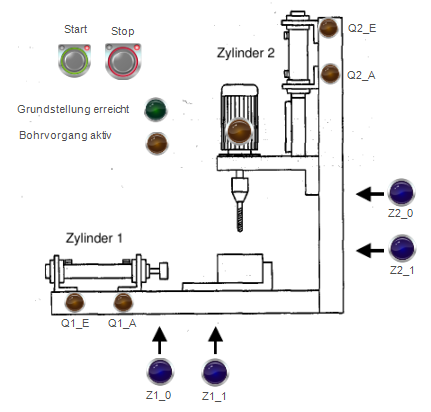
\includegraphics[scale=1]{Bilder/Simulation_Design.png}
    \caption[Design der Simulation]{Design der Simulation \footnotemark}
    \label{fig:Simulation}
\end{figure}
\footnotetext{\cite[in Anlehnung an][]{Riege}}   
Im oberen linken Bereich sind die Taster zur Steuerung der Bohrvorrichtung angebracht. Start entspricht dem Schalter \textit{S1}, Stop entspricht \textit{S2}. Darunter sind zwei \acp{led} zu sehen, die entsprechend der Betriebszustände aktiv sind. An den Zylindern sind jeweils zwei gelb leuchtende Kontroll-\ac{led} zu sehen. Diese sind aktiv, wenn der jeweilige Zylinder ein oder aus fährt. An der Antriebseinheit ist ebenso eine gelbe \ac{led} angebracht, die bei drehendem Bohrer leuchtet. Die Endanschläge der Zylinder, welche durch Sensoren erfasst werden, sind in der Simulation als blaue Leuchtmittel visuell dargestellt. Bei Erreichen der entsprechenden Stellung wird die dazugehörige \ac{led} eingeschaltet. Durch die Wahl ist zu jedem Zeitpunkt nachvollziehbar, in welchem Betriebszustand die Maschine ist und ob die Schrittkette korrekt abläuft.\\
Damit die Simulation lauffähig ist, müssen in den globalen Variablenlisten die Adressen der einzelnen Variablen auskommentiert werden. Treten bei der Simulation Fehler im Ablauf ab, muss das Hauptprogramm entsprechend verbessert werden. In der hier erstellten Steuerung ist das nicht der Fall. Der Programmablauf entspricht der vorher festgelegten Ablaufstruktur. Somit kann in einem möglichen nächsten Schritt das Programm auf eine reale \ac{sps} übertragen werden. Hierbei ist zu beachten, dass die deklarierten Adressen der einzelnen Sensoren und Aktoren auch mit der real verkabelten Bohreinrichtung übereinstimmt.